\documentclass[tikz,border=1mm,convert={outfile=\jobname.png}]{standalone}
\documentclass[tikz,border=5mm]{standalone}
\usepackage[utf8]{vietnam}
\usepackage{tikz,tkz-tab}
\usetikzlibrary{calc,3d}
%==============
\begin{document}
	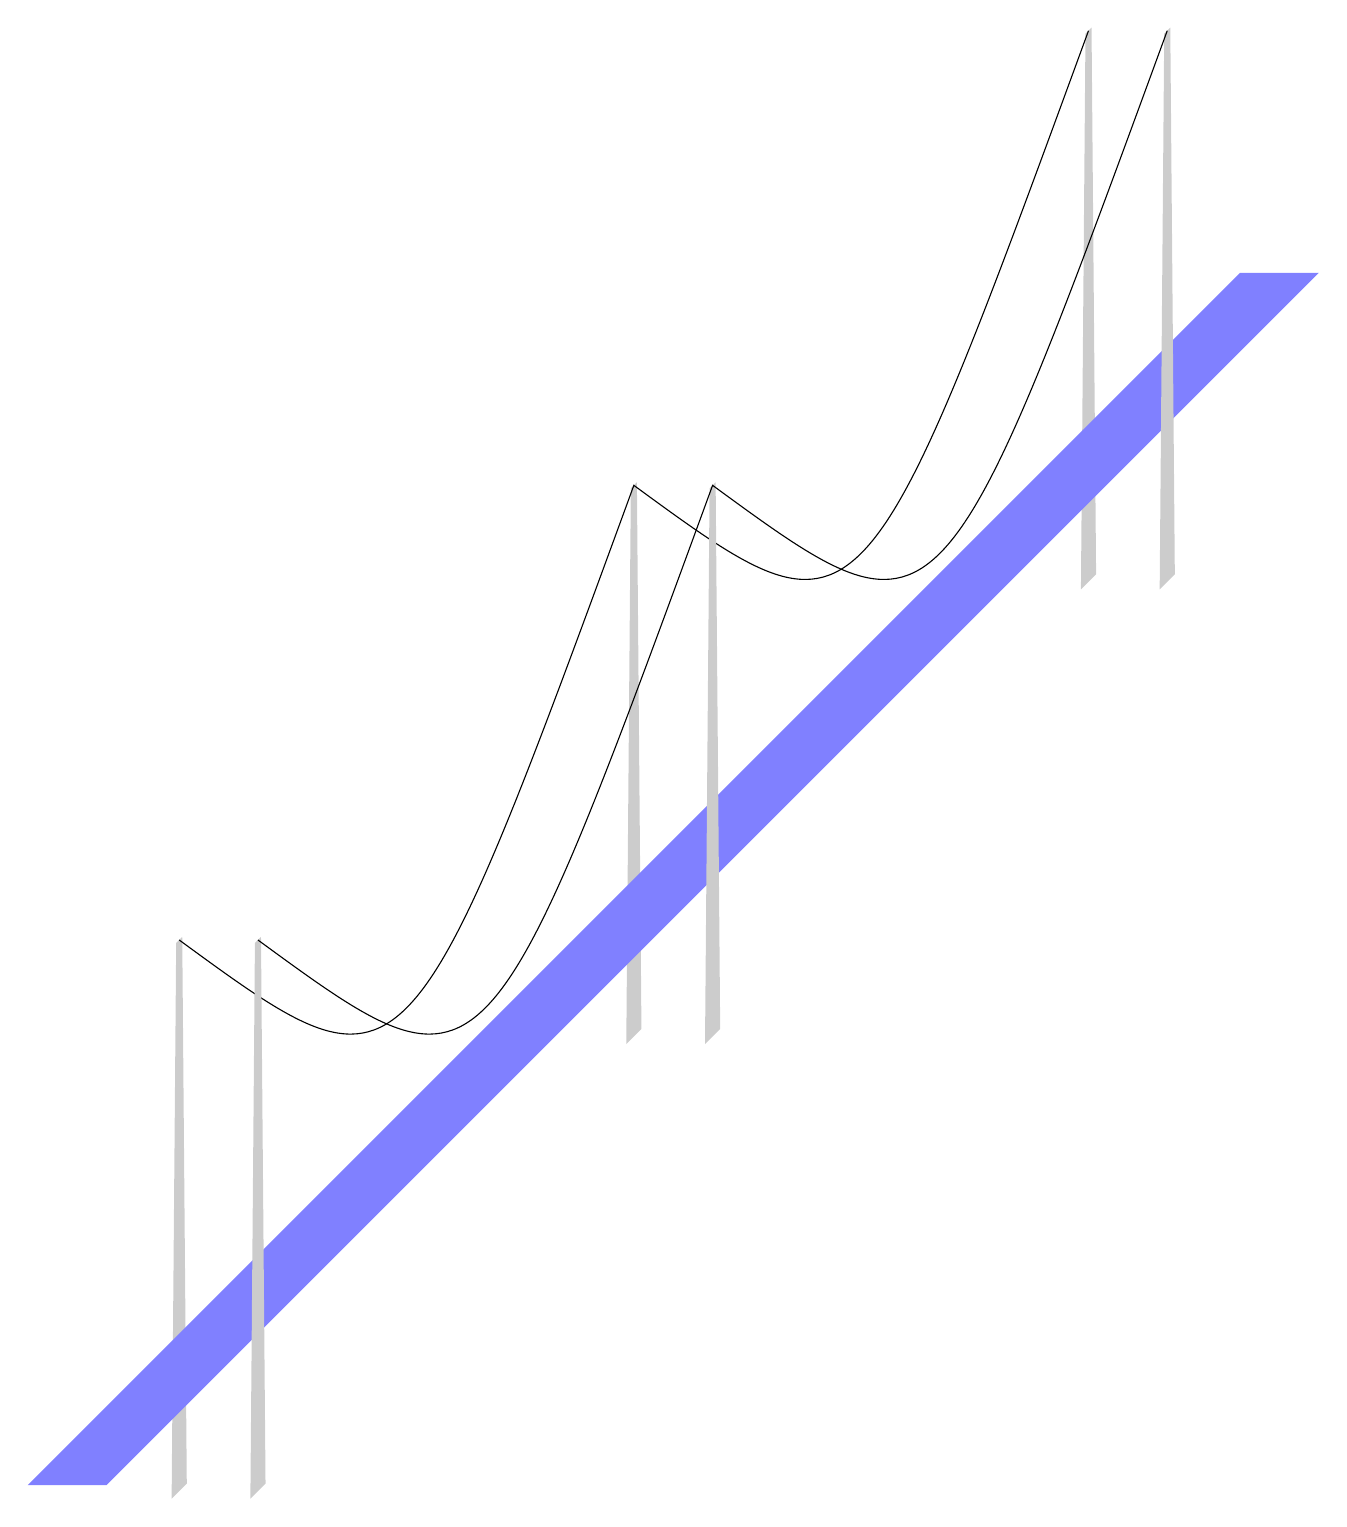
\begin{tikzpicture}
		\begin{scope}[canvas is yz plane at x=-0.5]
			\fill[gray!40] (-2,-0.25)--(5,-0.1)--(5,0.1)--(-2,0.25)--cycle;
			\fill[gray!40,shift={(0,15)}] (-2,-0.25)--(5,-0.1)--(5,0.1)--(-2,0.25)--cycle;
			\fill[gray!40,shift={(0,-15)}] (-2,-0.25)--(5,-0.1)--(5,0.1)--(-2,0.25)--cycle;
			\draw (5,-15) .. controls (0,-7.5)..(5,0) .. controls (0,7.5)..(5,15);
		\end{scope}
		\begin{scope}[canvas is xz plane at y=0]
			\fill[blue!50] (0.5,20)--(0.5,-20)--(-0.5,-20)--(-0.5,20)--cycle;
		\end{scope}
		\begin{scope}[canvas is yz plane at x=0.5]
			\fill[gray!40] (-2,-0.25)--(5,-0.1)--(5,0.1)--(-2,0.25)--cycle;
			\fill[gray!40,shift={(0,15)}] (-2,-0.25)--(5,-0.1)--(5,0.1)--(-2,0.25)--cycle;
			\fill[gray!40,shift={(0,-15)}] (-2,-0.25)--(5,-0.1)--(5,0.1)--(-2,0.25)--cycle;
			\draw (5,-15) .. controls (0,-7.5)..(5,0) .. controls (0,7.5)..(5,15);
		\end{scope}
	\end{tikzpicture}
\end{document}